\documentclass[letterpaper]{article}
\usepackage{graphicx}
\begin{document}

\title{Multicast File Transfer Protocol}
\author{Adam Drescher \and Magdalena Cassel}
\date{}

\maketitle

\begin{abstract}
In an effort to be portable, system developers often favor existing architectures, languages, operating systems, and standard libraries.
The dominant abstraction in established computing technologies for concurrency and therefore distributed system development is threads.
Consequently, distributed system developers are locked into using threads and experience the difficulties of thread-based development including obscure race conditions, poor support for the semantics of distributed systems, and difficulties integrating software developed using different thread models.
Furthermore, the demand for portability and generality dismisses many of the techniques proposed in research that involve new programming languages, language extensions, or domain-specific solutions.
This paper presents a development framework based on the I/O automata formal model implemented in C++.
The I/O automata model is a proven technique for distributed system design because its semantics match those found in distributed systems.
With the framework, developers can reason about correctness directly from the program text using the I/O automata formalism.
The I/O  automata model also provides a common abstraction for concurrency which facilitates software integration and promotes reuse.
TODO:  What are we doing for evaluation?
%% Our ability to realize sophisticated distributed systems such as those in cyber-physical systems and pervasive computing is predicated on a solid model and implementation of asynchrony and concurrency.
%% Threads, the de facto standard in practice, are not a suitable foundation because 1) ad hoc communication among threads prohibits software reuse, 2) threads are difficult to treat formally and therefore \emph{very} difficult to treat informally, and 3) threads are ill-suited for the asynchronous semantics present in the systems we desire to build.
%% In this paper, we outline the semantics necessary for building sophisticated distributed systems and connect these to the I/O automata formal model.
%% We then describe an implementation of the I/O automata formal model and cover extensions to the model necessary for operating in a dynamic environment.
%% Finally, we conclude with an evaluation of our I/O automata framework.
\end{abstract}

\section{Introduction}
% jrw:  Move this to the introduction.
Moving data across a network can take a variety of forms. These forms correspond to different user needs and consequently different protocols. Multicast File Transfer Protocol (MFTP) addresses the need to move immutable data between many different nodes in a fully distributed network. 
%% This is useful for 1) device discovery 2) File transfer in the absence of many technologies (including internet). the only thing that is necessary is computers with routing and broadcast/multicast enabled 3) maximizing the reach of a gossip style network

Advances in embedded systems and networking are paving the way for distributed systems of unprecedented sophistication.
Cyber-physical systems go beyond the traditional embedded system paradigm by explicitly modeling the dynamics of the physical system and communication network in the computational task.
The inclusion of wireless network interfaces in modern electronic devices is transforming our homes, offices, and hospitals into pervasive computing environments.
The interactions these systems have with the physical environment and its community of users require a degree of interoperability, configurability, adaptability, scalability, robustness, and security not found in existing systems.

One of the forces that prevents the development of any kind of sophisticated software system is accidental complexity~\cite{brooks_nsb}.
In the context of distributed systems, a major source of accidental complexity is a mismatch between the conceptual model of the system and the technology used to implement the system.
The mismatch between the conceptual model and implementation method introduces defects due to translation errors, slows rapid prototyping, and retards iterative refinement.
While there is no ``silver bullet''~\cite{brooks_nsb}, reducing the accidental complexity derived from the mismatch between concept and implementation will increase productivity and make new levels of sophistication possible with existing levels of effort.

Threads are the de facto implementation vehicle for most of computing including distributed systems.
Threads dominate because modern processors, programming languages, and operating systems were all developed to support the thread model.
Furthermore, the widespread availability of thread libraries makes them a natural choice for system development.
While threads dominate in practice, using threads to develop systems has a number of significant drawbacks.

First, ad hoc communication among threads prohibits software reuse.
To illustrate this problem consider the challenge of developing an application with a graphical user interface that also uses a multi-threaded middleware library.
Graphical user interfaces often use a single-threaded event-based design, e.g., X, Swing.
The system integrator must write glue code that bridges the single-threaded event-based semantics to multi-threaded semantics.
Bridging between two thread models is achievable, however, the systems we desire to build will rely on many libraries each with their own thread model.
The importance of a unified approach to concurrency becomes apparent when one considers bridging between different threading models, e.g., event-based, reactor, proactor, active objects, and their attributes, e.g., priority, thread-creation, blocking vs. non-blocking I/O.

Second, threads are difficult to treat formally and therefore \emph{very} difficult to treat informally.
The correctness of programs is reasoned about either formally as part of formal software design and verification and/or informally during the debugging process.
Since most programs will never be formally verified, the correctness of most programs hinges solely on the developers ability to reason about the program.
Based on the historical example of structured programming~\cite{goto_considered_harmful}, there is a strong correlation between what is ``easy'' in the formal arena and what is ``easy'' in the informal arena, especially when the implementation mimics the formal model, e.g., structured programming languages.
It is well known that a formal treatment of threads is difficult due to the arbitrary interleaving of critical sections and ability to define critical sections of arbitrary scope~\cite{lee_threads}.
Thus, the correctness of most multi-threaded programs hinges on the developer's ability to explore arbitrary interleavings of critical sections, i.e., model checking, in their head.

Third, threads are ill-suited for the asynchronous semantics present in the systems we desire to build.
The distributed systems we desire to build are asynchronous at both the device and network levels.
Embedded devices must respond to asynchronous events in the environment.
The interrupt-driven TinyOS operating system for wireless sensor network motes is an exemplar in this area.
The fundamental communication primitive in real-world distributed systems is asynchronous message passing.
Realizing asynchrony in a threaded program requires the use of signals (interrupts) and/or (a)synchronous I/O multiplexing.
Signals are primitive, rigid, and difficult to use correctly.
Synchronous I/O multiplexing, e.g., a select loop, is limited to operating system abstractions, e.g., file descriptors, and induces a reactive state machine structure that is difficult to understand and maintain.
Asynchronous I/O improves efficiency by avoiding the dispatching necessary to determine the I/O operation but are subject to the same limitations of shared-state thread-based programming.

Difficulties in developing asynchronous and concurrent software using threads has prompted a number of concurrent programming languages, e.g., Esterel, Erlang, Ptolemy, Autopipe, and language extensions, e.g., OpenMP, Cilk, Split-C.
Solutions that involve creating a new language or extending an existing language suffer from two main problems.
First, such solutions are often domain-specific and do not generalize to different applications, a necessity for heterogeneous distributed systems.
Furthermore, solutions not connected to a general-purpose formal model lack the important property that the complete system including the environment can be modeled as another component.
Second, such solutions often fail to become mainstream due to practical considerations.
For example, the combination of C and pthreads is much more popular than Erlang due to the popularity of C-like languages and C's connection with UNIX operating system.
Most language extensions are targeted at niche markets and therefore never standardized and implemented in mainstream compilers.

Thus, in order to build sophisticated distributed systems, we require a common semantics and model for building concurrent and asynchronous systems with straight-forward abstractions.
%% The model must be general to support the wide variety of devices and protocols necessary for cyber-physical and pervasive computing systems.
%% The model must facilitate the development of concurrent modules that can be reused.
%% The model must have a strong connection with a formal model to simplify the task of reasoning about individual components and complete systems.
%% The model must be implemented in such a way that it is easily approachable.
In section~\ref{system_model}, we expound upon the requirements of the model and connect the requirements with the I/O automata formal model.
Section~\ref{representation} describes how I/O automata are represented in our I/O automata framework.
In section~\ref{design}, we describe the design and implementation of our I/O automata framework.
Section~\ref{evaluation} provides an evaluation and discussion of our framework.
Section~\ref{related_work} contains an overview of related work and we offer our conclusions and thoughts for future work in section~\ref{conclusion}.

%% We provide a common semantics and model for building concurrent and asynchronous systems with straight-forward abstractions.

%%formal models, e.g., UNITY, I/O Automata,

%% Devices are asynchronous and concurrent.
%% Networks are asynchronous and concurrent.
%% Why not start with a model that is asynchronous and concurrent?

%% What inspires us:
%% \begin{itemize}
%%   \item CORBA - Remote Method Invocation (Remote Procedure Call with a ``this'' pointer).
%%     ``Let's make synchronous function calls over a network.''
%%     Assumes a thread of control.
%%     Asynchronous calls were added later (Did these result in obfuscation?)

%%   \item Patterns for asynchronous concurrency in a synchronous, thread-based world: Active objects, Reactor, Proactor, etc.
%%     Examples: X server, OS2 Presentation Manager, Java Swing

%%   \item AJAX - The modern Web is built on JavaScript + \emph{asynchronous} web page requests = AJAX.

%%   \item Michi Henning - ICE

%%   \item Steve Vinoski - Toolbox of programming languages

%% \end{itemize}

%% We provide a common semantics and model for building concurrent and asynchronous systems with straight-forward abstractions.

\pagebreak

\section{Model\label{model}}

\paragraph {Files.}
The main concept in MFTP is that of a \emph{file}.
Files are a sequence of bytes with a length and a user-defined type.
They are broken down into equally sized pieces called \emph{fragments}.  
Each file is uniquely identified by its \emph{file ID}, a structure that contains a hash of the file content, the file's length, and the file's type.
Given two files $f_1$ and $f_2$, one can define a matching predicate $\mu$.

\paragraph{Messages.}
File transfer takes place via \emph{messages}.
There are three types of messages in the protocol.
The first message type is a \emph{request}.
A request contains a file ID and a set of fragment indices.
We implemented requests as the file ID and a set of contiguous regions.  
However, one can envision the request to contain anything that defines a set.
The second message type is a \emph{fragment}, which consists of a file ID, a fragment index, and the data comprising that fragment of the file.
Last is a \emph{match}, which consists of a file ID and a set of matching file IDs.

\paragraph {Tasks.}
MFTP is a peer-to-peer protocol because each participant can act as both a client and a server.
A peer can send out any fragments for which it gets a request.
Fragments are periodically broadcast, even in the absence of requests, to indicate what files exist in the network.
A peer can use requests to poll for fragments of a file which can span from individual fragments to the whole file.
A peer which has successfully downloaded any number of fragments of a file can then serve those fragments.

Matching is a two-step process.
The first step applies a matching function $\iota$ to two file IDs to determine whether a match is possible between the two files.  
The second step applies a matching function $\mu$ to the two files to determine whether there is a match.
If $\mu$($f_1$,$f_2$) is true, $\iota$($fid_1$,$fid_2$) must be true.
However, if $\iota$($fid_1$,$fid_2$) is true, $\mu$($f_1$,$f_2$) does \emph{not} have to be true. 

%%TODO: Talk about validation

\section{Implementation}

%%TODO: Talk about validation - possible coinage 'incremental digest'

\paragraph{MFTP Automaton.}
Our implementation of MFTP uses the ioa framework.
I/O Automata model stateful distributed system components that can interact and be composed with each other.
They change state through transitions classified as input, output or internal actions.
Input and output actions in different automata are bound; output actions in the one trigger input actions in the other.

%%Describe our implementation at the 50k ft view and work our way down until things are no longer interesting.
We define a basic MFTP automaton, a sender, and a receiver.
The responsibilities of the MFTP automaton are to acquire data and to help others acquire it.
Each MFTP automaton begins with a file, encapsulated in a File object, which is either incomplete or complete.
If the file is incomplete, the automaton generates requests for the missing fragments.
If the file is complete, the automaton may serve the file, or it may serve the file while performing matching on it.

%%Picture of mFTP automaton?

MFTP automata receive messages via the receive input action.
If the input message is a valid fragment of its own file, the automaton saves the fragment.
If the input message is a request for fragments of its file, it flags those fragments as having been requested.
If the input message is a match containing its file ID, it records the matching IDs for download.

The automaton holds a queue of one message to send. 
The internal actions which fill this queue are triggered periodically.
The automaton generates messages containing one requested fragment if any fragments in the file have been requested.
The fragment sent is selected at random to help avoid collisions with other MFTP automata serving the same file.
The automaton generates requests if some fragments in the automaton's own file are missing.
The automaton generates match messages if it has recorded any matches to its file.

The automaton reports that its file is complete using the download complete output action.

\paragraph{Matching.}
Each MFTP automaton contains a flag that determines whether it will perform matching. 
It has another flag that determines whether it will self-destruct when it has finished downloading its file.
If the matching flag is set, the automaton applies the matching function $\iota$ to the file IDs of incoming fragments.
If $\iota$ is true, the automaton recursively constructs another MFTP automaton to download the potential match.
This child automaton does not perform matching.  
Its self-destruct flag is set so that it will self-destruct once the potential match has been downloaded.
When the download is complete, the parent automaton applies the matching function $\mu$ to the file to determine whether it is a match.

\paragraph{Some useful stuff.} %% We know it's rough, but what else can we do?
The sending automaton uses the UDP sender built into ioa to multicast messages one at a time.
The receiving automaton uses the ioa UDP receiver.
The sender and receiver automata may be connected to more than one MFTP automaton.

\vspace{5mm}
\includegraphics[scale=0.65]{diagramOne}

\paragraph{Jam.} %%needs different header
Our implementation defines three file types, \emph{data}, \emph{meta} and \emph{query}.  
A data file contains data from any file in the network.
A meta file contains as data the file ID of a file in the network and its name. 
A query file contains only the name of the file which is being queried.

We wrote two programs, \emph{Share} and \emph{Get}, which use MFTP, sender and receiver automata to disseminate a file or files. %%Can one 'disseminate' a file?
Share creates two MFTP automata, \emph{file server} and \emph{meta server}.
File server is constructed with a complete file \emph{f}, and meta server is constructed with a meta file.
The meta file is generated from the fileID and name of f.
At the start, Get creates one MFTP automaton, \emph{query server}, constructed with a query file.
The query file is generated from the name of the file to download, supplied by a command line argument.

We defined a functor interface so that Share and Get could use different $\iota$ and $\mu$ functions.
In Share, meta server performs matching on the meta file and broadcasts matches to f.
Its $\iota$ returns true if the incoming file is a query file.
Its $\mu$ returns true if the contents of the downloaded query file match the name of f.

\vspace{2 mm}

\includegraphics[scale=0.55]{share_diagram}

\vspace{2 mm}

In Get, query server performs matching on the query file.
Its $\iota$ returns true if the incoming file is a meta file.
Its $\mu$ returns true if the contents of the downloaded meta file match the name of the file being queried.
Query server passes the meta files downloaded by its child automata to Get.
Using the file IDs contained in the meta files, Get constructs further MFTP automata which download the files pertaining to those file IDs.

\vspace{2.5 mm}

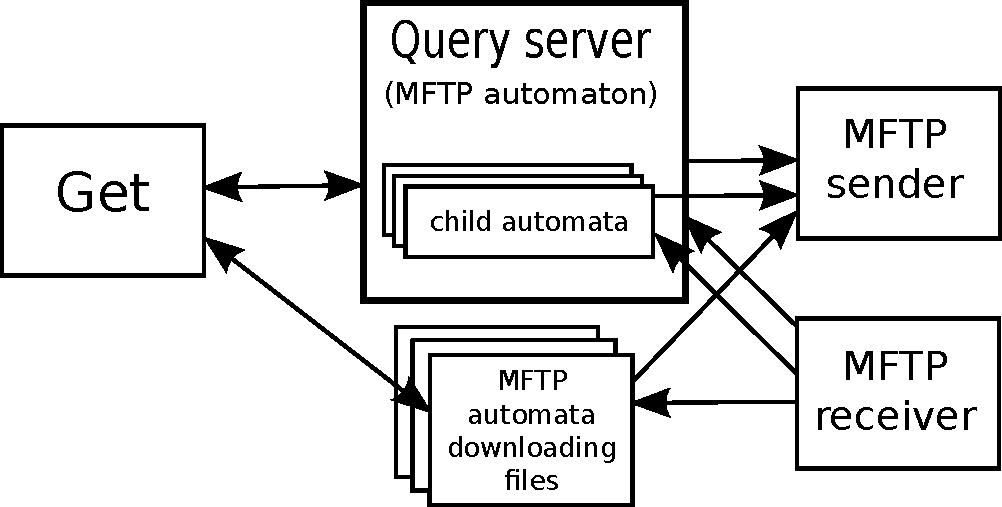
\includegraphics[scale=0.65]{get_diagram}

\vspace{2 mm}

%%\begin{itemize}
%%  \item Problem
%%  \item Design forces
%%  \item Solution
%%  \item Consequences
%%\end{itemize}

\section{Evaluation and Discussion\label{evaluation}}

\begin{itemize}
\item Translation of automaton in \emph{Distributed Algorithms} to C++.
\item Simulate a protocol then replace with network components
\item Compare a protocol using: single-threaded event-based (select loop), multi-threaded, I/O automata
\item Show a buggy program and then apply an invariant to find the bug.
\end{itemize}

Bring up style mentioned in section \ref{representation}.

\section{Related Work\label{related_work}}

pthreads (?)
Edward Lee - The Problem with Threads
Herb Sutter - The Free Lunch is Over
Early work on concurrency

\section{Conclusion and Future Work\label{conclusion}}

\begin{itemize}
  \item We are going to use it to build the substrate.
  \item Speculate on moving down into operating system (device drivers would be easy, IPC including filesystem replaced by automata)
  \item Speculate on moving down into the hardware level (Local talent, Ivan Sutherland)
  \item We can take advantage of multi-core in a very straight-forward way
  \item New problems in scheduling (Pinning automata to processors to minimize actions that span two processors.  Maximum independent set.)
  \item We are non-blocking all the way.  Combine this with a deterministic implementation of the scheduler and model and there are serious opportunities for real-time.
\end{itemize}

\end{document}
